\subsection{For Resten}
\label{subsec:forresten}

For Resten er en gratis mobilapp, der er udgivet af Forbrugerrådet som en del af en kampagne mod madspild. App’en findes til Android og iOS og kan installeres fra henholdsvis Google Play og App Store. App’en fungerer ved, at man på to ``hjul'' vælger kategori (``Kornprodukter'', ``Mejeriprodukter'', ``Kød og æg'' og fem andre kategorier) og rest (\fx ``Mørbrad'', ``Kylling'', ``Kødsovs'' osv.), hvorefter brugeren præsenteres for en række opskrifter, som inkluderer den valgte rest.

\begin{figure}[H]
\centering
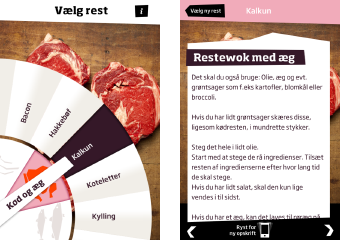
\includegraphics[scale=0.7]{billeder/forbilleder/forresten.png}
\capt{Brugergrænseflade i For Resten. Valg af rest (t.v.) og visning af opskrift (t.h.)}
\label{fig:forresten}
\end{figure}

For hver rest er der ca. 4 - 5 opskrifter, hvilket med 124 rester giver et samlet antal opskrifter på omkring 500 - 600 (dette er vores eget bud på mængden. Det faktiske antal opskrifter er ikke oplyst nogen steder). For opskrifterne vises der kun fremgangsmåde, og ikke en liste over ingredienser. Det er derfor heller ikke muligt at op- eller nedskalere opskrifsportionerne. Derudover er der ingen mulighed for at favorisere opskrifter eller på anden måde gemme resultater af en søgning. I forhold til søgningen så kan man, som sagt, kun søge på én enkelt rest, og ikke sammensætte rester, som ved andre løsninger. Samtidig har man kun mulighed for at vælge sin rest på hjulene, og har altså ikke muligheden for at skrive i et felt. Under afprøvningen var det derfor i nogle tilfælde svært at finde den ønskede ingrediens. Det er de samme problemstillinger, der kommer til udtryk i brugernes anmeldelser af app’en på Google Play. \Fx skriver brugeren \textit{TJA} \cite{tja}:

\begin{quote}
``Fin ide, men den burde være blevet kælet lidt mere for, før den røg i play. Hvem laver restemad af én rest og så en masse ting der skal købes? Jeg har brug for at kunne søge på tre-fire rester for at se, hvordan de kan kombineres til noget spændende. Og hvis jeg finder en opskrift, jeg vil prøve, så kan jeg ikke gemme den i appen, men skal søge den frem igen når jeg står i netto og skal købe de ting, der skal til - og søge den frem igen, når jeg skal lave maden. Alt for besværligt.''
\end{quote}

Sammenlagt har app’en på Google Play bedømmelsen 2,4 stjerner ud af 5, baseret på 69 bedømmelser, hvoraf næsten halvdelen kun har givet app’en 1 stjerne. Et andet kritikpunkt, der kommer til udtryk i flere anmeldelser, er, at app’en bruger for mange systemressourcer og er langsom til at starte op.
